\documentclass{standalone}
\usepackage{tikz}
\usetikzlibrary{patterns, positioning}


\begin{document}
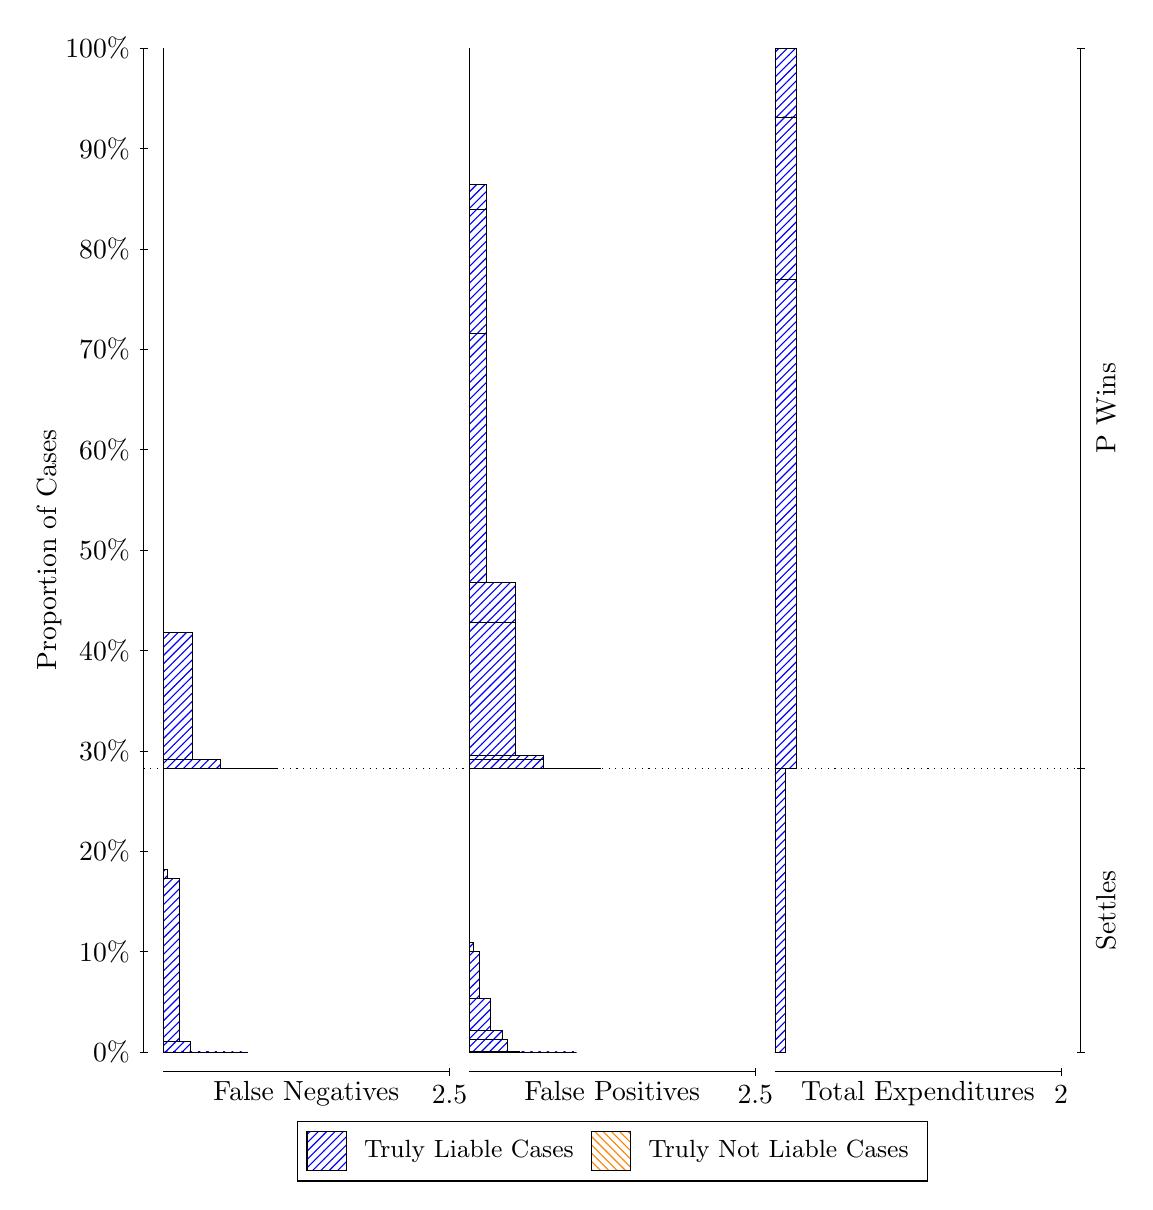
\begin{tikzpicture}
\draw[black, very thin] (1.5,1.75) -- (1.5,14.5);
\node[rotate=90, text=black, anchor=center] at (0.3, 8.125) {Proportion of Cases};
\draw[black, very thin] (1.45,1.75) -- (1.55,1.75);
\node[text=black, anchor=east] at (1.45, 1.75) {0\%};
\draw[black, very thin] (1.45,3.025) -- (1.55,3.025);
\node[text=black, anchor=east] at (1.45, 3.025) {10\%};
\draw[black, very thin] (1.45,4.3) -- (1.55,4.3);
\node[text=black, anchor=east] at (1.45, 4.3) {20\%};
\draw[black, very thin] (1.45,5.575) -- (1.55,5.575);
\node[text=black, anchor=east] at (1.45, 5.575) {30\%};
\draw[black, very thin] (1.45,6.85) -- (1.55,6.85);
\node[text=black, anchor=east] at (1.45, 6.85) {40\%};
\draw[black, very thin] (1.45,8.125) -- (1.55,8.125);
\node[text=black, anchor=east] at (1.45, 8.125) {50\%};
\draw[black, very thin] (1.45,9.4) -- (1.55,9.4);
\node[text=black, anchor=east] at (1.45, 9.4) {60\%};
\draw[black, very thin] (1.45,10.675) -- (1.55,10.675);
\node[text=black, anchor=east] at (1.45, 10.675) {70\%};
\draw[black, very thin] (1.45,11.95) -- (1.55,11.95);
\node[text=black, anchor=east] at (1.45, 11.95) {80\%};
\draw[black, very thin] (1.45,13.225) -- (1.55,13.225);
\node[text=black, anchor=east] at (1.45, 13.225) {90\%};
\draw[black, very thin] (1.45,14.5) -- (1.55,14.5);
\node[text=black, anchor=east] at (1.45, 14.5) {100\%};

\draw[black, very thin] (13.4,1.75) -- (13.4,14.5);
\draw[black, very thin] (13.35,1.75) -- (13.45,1.75);
\node[anchor=west] at (13.35, 1.75) {};
\draw[black, very thin] (13.35,5.3513) -- (13.45,5.3513);
\node[anchor=west] at (13.35, 5.3513) {};
\draw[black, very thin] (13.35,14.5) -- (13.45,14.5);
\node[anchor=west] at (13.35, 14.5) {};

\draw[black, very thin, pattern color=blue, pattern=north east lines] (1.75,1.75) rectangle (2.8218,1.75);
\draw[black, very thin, pattern color=blue, pattern=north east lines] (1.75,1.75) rectangle (2.5312,1.75);
\draw[black, very thin, pattern color=blue, pattern=north east lines] (1.75,1.75) rectangle (2.4585,1.751);
\draw[black, very thin, pattern color=blue, pattern=north east lines] (1.75,1.751) rectangle (2.3858,1.751);
\draw[black, very thin, pattern color=blue, pattern=north east lines] (1.75,1.751) rectangle (2.2405,1.751);
\draw[black, very thin, pattern color=blue, pattern=north east lines] (1.75,1.751) rectangle (2.1678,1.7519);
\draw[black, very thin, pattern color=blue, pattern=north east lines] (1.75,1.7519) rectangle (2.0952,1.8864);
\draw[black, very thin, pattern color=blue, pattern=north east lines] (1.75,1.8864) rectangle (2.0225,1.8866);
\draw[black, very thin, pattern color=blue, pattern=north east lines] (1.75,1.8866) rectangle (1.9498,3.9557);
\draw[black, very thin, pattern color=blue, pattern=north east lines] (1.75,3.9557) rectangle (1.8772,3.9559);
\draw[black, very thin, pattern color=blue, pattern=north east lines] (1.75,3.9559) rectangle (1.8045,4.0692);
\draw[black, very thin, pattern color=orange, pattern=north west lines] (1.75,4.0692) rectangle (1.75,4.0692);
\draw[black, very thin, pattern color=blue, pattern=north east lines] (1.75,4.0692) rectangle (1.75,5.3513);
\draw[black, very thin, pattern color=blue, pattern=north east lines] (1.75,5.3513) rectangle (3.2033,5.3513);
\draw[black, very thin, pattern color=blue, pattern=north east lines] (1.75,5.3513) rectangle (2.84,5.3525);
\draw[black, very thin, pattern color=blue, pattern=north east lines] (1.75,5.3525) rectangle (2.4767,5.4672);
\draw[black, very thin, pattern color=blue, pattern=north east lines] (1.75,5.4672) rectangle (2.1133,7.0794);
\draw[black, very thin, pattern color=orange, pattern=north west lines] (1.75,7.0794) rectangle (1.75,7.0794);
\draw[black, very thin, pattern color=blue, pattern=north east lines] (1.75,7.0794) rectangle (1.75,14.5);
\draw[black, very thin, pattern color=orange, pattern=north west lines] (5.6333,1.75) rectangle (6.9958,1.75);
\draw[black, very thin, pattern color=blue, pattern=north east lines] (5.6333,1.75) rectangle (6.9958,1.75);
\draw[black, very thin, pattern color=orange, pattern=north west lines] (5.6333,1.75) rectangle (6.7052,1.75);
\draw[black, very thin, pattern color=blue, pattern=north east lines] (5.6333,1.75) rectangle (6.7052,1.75);
\draw[black, very thin, pattern color=blue, pattern=north east lines] (5.6333,1.75) rectangle (6.6325,1.75);
\draw[black, very thin, pattern color=orange, pattern=north west lines] (5.6333,1.75) rectangle (6.5598,1.75);
\draw[black, very thin, pattern color=blue, pattern=north east lines] (5.6333,1.75) rectangle (6.5598,1.75);
\draw[black, very thin, pattern color=orange, pattern=north west lines] (5.6333,1.75) rectangle (6.4145,1.75);
\draw[black, very thin, pattern color=blue, pattern=north east lines] (5.6333,1.75) rectangle (6.4145,1.7514);
\draw[black, very thin, pattern color=blue, pattern=north east lines] (5.6333,1.7514) rectangle (6.3418,1.7514);
\draw[black, very thin, pattern color=blue, pattern=north east lines] (5.6333,1.7514) rectangle (6.2692,1.7544);
\draw[black, very thin, pattern color=blue, pattern=north east lines] (5.6333,1.7544) rectangle (6.1965,1.7544);
\draw[black, very thin, pattern color=orange, pattern=north west lines] (5.6333,1.7544) rectangle (6.1238,1.7544);
\draw[black, very thin, pattern color=blue, pattern=north east lines] (5.6333,1.7544) rectangle (6.1238,1.9145);
\draw[black, very thin, pattern color=blue, pattern=north east lines] (5.6333,1.9145) rectangle (6.0512,2.0281);
\draw[black, very thin, pattern color=blue, pattern=north east lines] (5.6333,2.0281) rectangle (5.9785,2.0282);
\draw[black, very thin, pattern color=blue, pattern=north east lines] (5.6333,2.0282) rectangle (5.9058,2.4296);
\draw[black, very thin, pattern color=blue, pattern=north east lines] (5.6333,2.4296) rectangle (5.8332,2.4298);
\draw[black, very thin, pattern color=blue, pattern=north east lines] (5.6333,2.4298) rectangle (5.7605,3.0321);
\draw[black, very thin, pattern color=blue, pattern=north east lines] (5.6333,3.0321) rectangle (5.6878,3.1454);
\draw[black, very thin, pattern color=blue, pattern=north east lines] (5.6333,3.1454) rectangle (5.6333,5.3513);
\draw[black, very thin, pattern color=orange, pattern=north west lines] (5.6333,5.3513) rectangle (7.3047,5.3513);
\draw[black, very thin, pattern color=blue, pattern=north east lines] (5.6333,5.3513) rectangle (7.3047,5.3513);
\draw[black, very thin, pattern color=orange, pattern=north west lines] (5.6333,5.3513) rectangle (6.9413,5.3513);
\draw[black, very thin, pattern color=blue, pattern=north east lines] (5.6333,5.3513) rectangle (6.9413,5.3526);
\draw[black, very thin, pattern color=blue, pattern=north east lines] (5.6333,5.3526) rectangle (6.9413,5.3534);
\draw[black, very thin, pattern color=orange, pattern=north west lines] (5.6333,5.3534) rectangle (6.578,5.3534);
\draw[black, very thin, pattern color=blue, pattern=north east lines] (5.6333,5.3534) rectangle (6.578,5.4667);
\draw[black, very thin, pattern color=blue, pattern=north east lines] (5.6333,5.4667) rectangle (6.578,5.518);
\draw[black, very thin, pattern color=orange, pattern=north west lines] (5.6333,5.518) rectangle (6.2147,5.518);
\draw[black, very thin, pattern color=blue, pattern=north east lines] (5.6333,5.518) rectangle (6.2147,7.2119);
\draw[black, very thin, pattern color=blue, pattern=north east lines] (5.6333,7.2119) rectangle (6.2147,7.7165);
\draw[black, very thin, pattern color=blue, pattern=north east lines] (5.6333,7.7165) rectangle (5.8513,10.872);
\draw[black, very thin, pattern color=orange, pattern=north west lines] (5.6333,10.872) rectangle (5.8513,10.872);
\draw[black, very thin, pattern color=blue, pattern=north east lines] (5.6333,10.872) rectangle (5.8513,12.453);
\draw[black, very thin, pattern color=blue, pattern=north east lines] (5.6333,12.453) rectangle (5.8513,12.772);
\draw[black, very thin, pattern color=blue, pattern=north east lines] (5.6333,12.772) rectangle (5.6333,14.5);
\draw[black, very thin, pattern color=orange, pattern=north west lines] (9.5167,1.75) rectangle (9.6529,1.75);
\draw[black, very thin, pattern color=blue, pattern=north east lines] (9.5167,1.75) rectangle (9.6529,5.3513);
\draw[black, very thin, pattern color=orange, pattern=north west lines] (9.5167,5.3513) rectangle (9.7892,5.3513);
\draw[black, very thin, pattern color=blue, pattern=north east lines] (9.5167,5.3513) rectangle (9.7892,11.56);
\draw[black, very thin, pattern color=orange, pattern=north west lines] (9.5167,11.56) rectangle (9.7892,11.56);
\draw[black, very thin, pattern color=blue, pattern=north east lines] (9.5167,11.56) rectangle (9.7892,13.625);
\draw[black, very thin, pattern color=orange, pattern=north west lines] (9.5167,13.625) rectangle (9.7892,13.625);
\draw[black, very thin, pattern color=blue, pattern=north east lines] (9.5167,13.625) rectangle (9.7892,14.5);
\draw[black, dotted] (1.5,5.3513) -- (13.4,5.3513);
\draw[black, very thin] (1.75,1.5) -- (5.3833,1.5);
\node[text=black, anchor=north] at (3.5667, 1.5) {False Negatives};
\draw[black, very thin] (5.3833,1.45) -- (5.3833,1.55);
\node[text=black, anchor=north] at (5.3833, 1.45) {2.5};

\draw[black, very thin] (5.6333,1.5) -- (9.2667,1.5);
\node[text=black, anchor=north] at (7.45, 1.5) {False Positives};
\draw[black, very thin] (9.2667,1.45) -- (9.2667,1.55);
\node[text=black, anchor=north] at (9.2667, 1.45) {2.5};

\draw[black, very thin] (9.5167,1.5) -- (13.15,1.5);
\node[text=black, anchor=north] at (11.333, 1.5) {Total Expenditures};
\draw[black, very thin] (13.15,1.45) -- (13.15,1.55);
\node[text=black, anchor=north] at (13.15, 1.45) {2};

\node[text=black, centered, rotate=90] at (13.72, 3.5506) {Settles};
\node[text=black, centered, rotate=90] at (13.72, 9.9256) {P Wins};

\draw (7.449999999999999,1.5) node[draw=none] (baseCoordinate) {};
\begin{scope}[align=center]
        \matrix[scale=0.5, draw=black, below=0.5cm of baseCoordinate, nodes={draw}, column sep=0.1cm]{
            \node[rectangle, draw, minimum width=0.5cm, minimum height=0.5cm, pattern color=blue, pattern=north east lines] {}; &
            \node[draw=none, font=\small, text=black] (B) {Truly Liable Cases}; &
            \node[rectangle, draw, minimum width=0.5cm, minimum height=0.5cm, pattern color=orange, pattern=north west lines] {}; &
            \node[draw=none, font=\small, text=black] (B) {Truly Not Liable Cases}; \\
            };
\end{scope}

\end{tikzpicture}
\end{document}